% Options for packages loaded elsewhere
\PassOptionsToPackage{unicode}{hyperref}
\PassOptionsToPackage{hyphens}{url}
%
\documentclass[
  12pt,
]{article}
\usepackage{amsmath,amssymb}
\usepackage{iftex}
\ifPDFTeX
  \usepackage[T1]{fontenc}
  \usepackage[utf8]{inputenc}
  \usepackage{textcomp} % provide euro and other symbols
\else % if luatex or xetex
  \usepackage{unicode-math} % this also loads fontspec
  \defaultfontfeatures{Scale=MatchLowercase}
  \defaultfontfeatures[\rmfamily]{Ligatures=TeX,Scale=1}
\fi
\usepackage{lmodern}
\ifPDFTeX\else
  % xetex/luatex font selection
\fi
% Use upquote if available, for straight quotes in verbatim environments
\IfFileExists{upquote.sty}{\usepackage{upquote}}{}
\IfFileExists{microtype.sty}{% use microtype if available
  \usepackage[]{microtype}
  \UseMicrotypeSet[protrusion]{basicmath} % disable protrusion for tt fonts
}{}
\makeatletter
\@ifundefined{KOMAClassName}{% if non-KOMA class
  \IfFileExists{parskip.sty}{%
    \usepackage{parskip}
  }{% else
    \setlength{\parindent}{0pt}
    \setlength{\parskip}{6pt plus 2pt minus 1pt}}
}{% if KOMA class
  \KOMAoptions{parskip=half}}
\makeatother
\usepackage{xcolor}
\usepackage[margin=1in]{geometry}
\usepackage{longtable,booktabs,array}
\usepackage{calc} % for calculating minipage widths
% Correct order of tables after \paragraph or \subparagraph
\usepackage{etoolbox}
\makeatletter
\patchcmd\longtable{\par}{\if@noskipsec\mbox{}\fi\par}{}{}
\makeatother
% Allow footnotes in longtable head/foot
\IfFileExists{footnotehyper.sty}{\usepackage{footnotehyper}}{\usepackage{footnote}}
\makesavenoteenv{longtable}
\usepackage{graphicx}
\makeatletter
\def\maxwidth{\ifdim\Gin@nat@width>\linewidth\linewidth\else\Gin@nat@width\fi}
\def\maxheight{\ifdim\Gin@nat@height>\textheight\textheight\else\Gin@nat@height\fi}
\makeatother
% Scale images if necessary, so that they will not overflow the page
% margins by default, and it is still possible to overwrite the defaults
% using explicit options in \includegraphics[width, height, ...]{}
\setkeys{Gin}{width=\maxwidth,height=\maxheight,keepaspectratio}
% Set default figure placement to htbp
\makeatletter
\def\fps@figure{htbp}
\makeatother
\setlength{\emergencystretch}{3em} % prevent overfull lines
\providecommand{\tightlist}{%
  \setlength{\itemsep}{0pt}\setlength{\parskip}{0pt}}
\setcounter{secnumdepth}{5}
\newlength{\cslhangindent}
\setlength{\cslhangindent}{1.5em}
\newlength{\csllabelwidth}
\setlength{\csllabelwidth}{3em}
\newlength{\cslentryspacingunit} % times entry-spacing
\setlength{\cslentryspacingunit}{\parskip}
\newenvironment{CSLReferences}[2] % #1 hanging-ident, #2 entry spacing
 {% don't indent paragraphs
  \setlength{\parindent}{0pt}
  % turn on hanging indent if param 1 is 1
  \ifodd #1
  \let\oldpar\par
  \def\par{\hangindent=\cslhangindent\oldpar}
  \fi
  % set entry spacing
  \setlength{\parskip}{#2\cslentryspacingunit}
 }%
 {}
\usepackage{calc}
\newcommand{\CSLBlock}[1]{#1\hfill\break}
\newcommand{\CSLLeftMargin}[1]{\parbox[t]{\csllabelwidth}{#1}}
\newcommand{\CSLRightInline}[1]{\parbox[t]{\linewidth - \csllabelwidth}{#1}\break}
\newcommand{\CSLIndent}[1]{\hspace{\cslhangindent}#1}
\usepackage{setspace} \usepackage{lineno} \usepackage{placeins} \usepackage[nottoc,notlof,notlot]{tocbibind} \renewcommand{\contentsname}{} \renewcommand{\listfigurename}{} \renewcommand{\listtablename}{} \usepackage{sectsty} \sectionfont{\centering}
\usepackage{booktabs}
\usepackage{longtable}
\usepackage{array}
\usepackage{multirow}
\usepackage{wrapfig}
\usepackage{float}
\usepackage{colortbl}
\usepackage{pdflscape}
\usepackage{tabu}
\usepackage{threeparttable}
\usepackage{threeparttablex}
\usepackage[normalem]{ulem}
\usepackage{makecell}
\usepackage{xcolor}
\ifLuaTeX
  \usepackage{selnolig}  % disable illegal ligatures
\fi
\IfFileExists{bookmark.sty}{\usepackage{bookmark}}{\usepackage{hyperref}}
\IfFileExists{xurl.sty}{\usepackage{xurl}}{} % add URL line breaks if available
\urlstyle{same}
\hypersetup{
  hidelinks,
  pdfcreator={LaTeX via pandoc}}

\author{}
\date{\vspace{-2.5em}}

\begin{document}

\doublespacing

\begin{center}
    
\textbf{\Large Bibliometric Analysis of Mangroves in Fisheries}
    
\textsc{Sophie Wulfing$^{1*}$ and Rohani Ambo Rappe$^{1}$\\}
\vspace{3 mm}
\normalsize{\indent $^1$Department of Marine Ecology, Hasanuddin University, Indonesia\\}
$\text{*}$ Corresponding authors: Sophie Wulfing (SophieWulfing@gmail.com)
\end{center}

\newpage

\hypertarget{introduction}{%
\section{INTRODUCTION}\label{introduction}}

Mangroves are inter-tidal forests that are essential components to many tropical ecosystems. As the effects of climate change grow stronger worldwide, the need for carbon mitigation and protection against extreme weather are becoming more urgent. Mangroves are key actors in maintaining the biodiversity of the ecosystems they inhabit. Mangroves have been reported to support up 20\% of the benthic biodiversity in their habitats (Carugati et al., 2018). They provide essential nutrients, temperature controls, and protection from predators for marine life (Blue Forests, 2012). Further, Mangroves have been shown to increase fishery yields in their surrounding areas, therefore increasing fisher income (Aburto-Oropeza et al., 2008). The root systems of mangroves provide shelter and protection for juvenile fish, allowing them to grow and develop safely away from predators and also also act as a buffer against strong currents and waves, creating calmer and more stable environments where fish can feed and reproduce (Alongi, 2008). Areas with intact mangrove forests have been shown to support higher fish abundance and diversity compared to areas without mangroves (Nagelkerken et al., 2008). Mangroves provide a rich food web, with leaf litter and detritus serving as a source of nutrients that fuel the basis of the food chain, supporting the growth and survival of various fish species (Alongi, 2008). Furthermore, mangroves act as a buffer against coastal erosion and storm surges, safeguarding the habitats of both fish and fishermen (Nagelkerken et al., 2008). Mangroves offer a crucial line of defense against the impacts of climate change on fisheries. The dense root systems of mangroves stabilize shorelines and protect coastal areas from erosion caused by rising sea levels and extreme weather events (Alongi, 2008).

Mangroves biomes comprise about 14 \% of marine carbon sequestration and may result in high gas emissions when these ecosystems are disturbed (Alongi, 2012), while more established mangroves are more efficient in absorbing atmospheric carbon (Cameron et al., 2019). Despite all of their contributions to ecosystem health, mangrove environments are being threatened worldwide. Rising sea-levels has been shown to be a major contributor to mangrove loss (Gilman et al., 2008). Further, as extreme events are becoming more intense and more frequent, these could potentially threaten mangroves due to defoliation, soil erosion, or by altering the chemical makeup or temperature of soils (Gilman et al., 2008). Mangroves are also directly threatened by anthropogenic activity. Pollution, coastal development, and aquaculture development have also contributed to mangrove ecosystem loss (Adeel \& Pomeroy, 2002). Mangrove forests in the Western Tropical Pacific are the most diverse of these habitats globally (Ellison et al., 1999).

Anthropogenic activity provides a threat to mangroves as 210 million people worldwide live within 10 km mangroves. The largest single-driver of mangrove loss has been urban expansion or the development of aquaculture ponds. However, economic gains from these activities have been shown to be temporary or only benefiting small portions of the community (Hutchison \& Spalding, 2014). Therefore, the destruction of mangroves often leads to long term financial loss. Although the exact financial gain from fisheries dependent on mangroves is hard to measure world-wide, estimates of the finiancial contribution of mangroves to small scale fisheries has been shown to be as high as \$12,305 per hectare per year. (Hutchison \& Spalding, 2014). An estimated 4.1 million of fishers rely on mangrove-dependant fisheries, primarily in Indonesia, Bangladesh, Myanmar, and Brazil (Zu Ermgassen et al., 2021). Some of the countries with highest numbers of mangrove reliant fishers also have the highest dependence on these fisheries for essential sources of nutrition (Zu Ermgassen et al., 2021). Therefore, not only do mangroves provide essential climate change mitigation and protection against extreme weather, but are the base of of the foodweb for many essential fisheries around the globe and are a key actor in ensuring food security for many tropical communities.

Bibliometric analysis is a statistical analysis of trends in research related to a specific topic. It can identify the evolution of a scientific topic, as well as emerging questions and interests in the field. It can also be used to locate gaps in scientific knowledge in order to direct where future research should focus (Donthu et al., 2021). Bibliometric analysis is a useful tool to glean out high-impact research as well, and provide a baseline for which papers are highly cited and influential in a field of study (Ellegaard \& Wallin, 2015).

In this study, we aim to conduct a bibliometric analysis of research trends that connect mangroves to fisheries, particularly through the lense of biomass and biodiversity. Our goal of this research is to 1) identify which countries and journals have had the highest impact in this field of study 2) identify trends in keywords in order to identify what issues have driven the research of mangrove-dependent fisheries and 3) to assess the amount of cooperation and collaboration that is occurring in this field.

\hypertarget{methods}{%
\section{METHODS}\label{methods}}

Documents were collected using the Scopus database. The keywords ``Mangroves'', ``Fisheries'', and ``Biomass OR Biodiversity'' were used to conduct the search, and results were filtered to the following subject areas: Environmental Science, Agriculture and Biological Sciences, Earth and Planetary Sciences, Social Sciences, Economics Econometrics and Finance, Multidisciplinary, Energy, Computer Science, Mathematics, and Decision Sciences. A total of 251 articles were found from a total of 138 different sources, and results were limited to research articles so that SOMETHING SOMETHING SOMETHING. Information on WHICH BITS OF DATA DID YOU USE was collected on each paper to conduct bibliometric analysis.

Analysis

The search results were cleaned using OpenRefine CHECK OUT THIS WEBSITE website to avoid duplicate keywords with the same meanings. VOSviewer and Tableau were used in the visualizations of XYZ MAKE SOME MORE HERE I GUESS AND HAVE CITATION. Further the R package Bibliometrix (CITATION) was used to make THE FIGURES BLAH BLAH

\hypertarget{results}{%
\section{RESULTS}\label{results}}

\begin{figure}
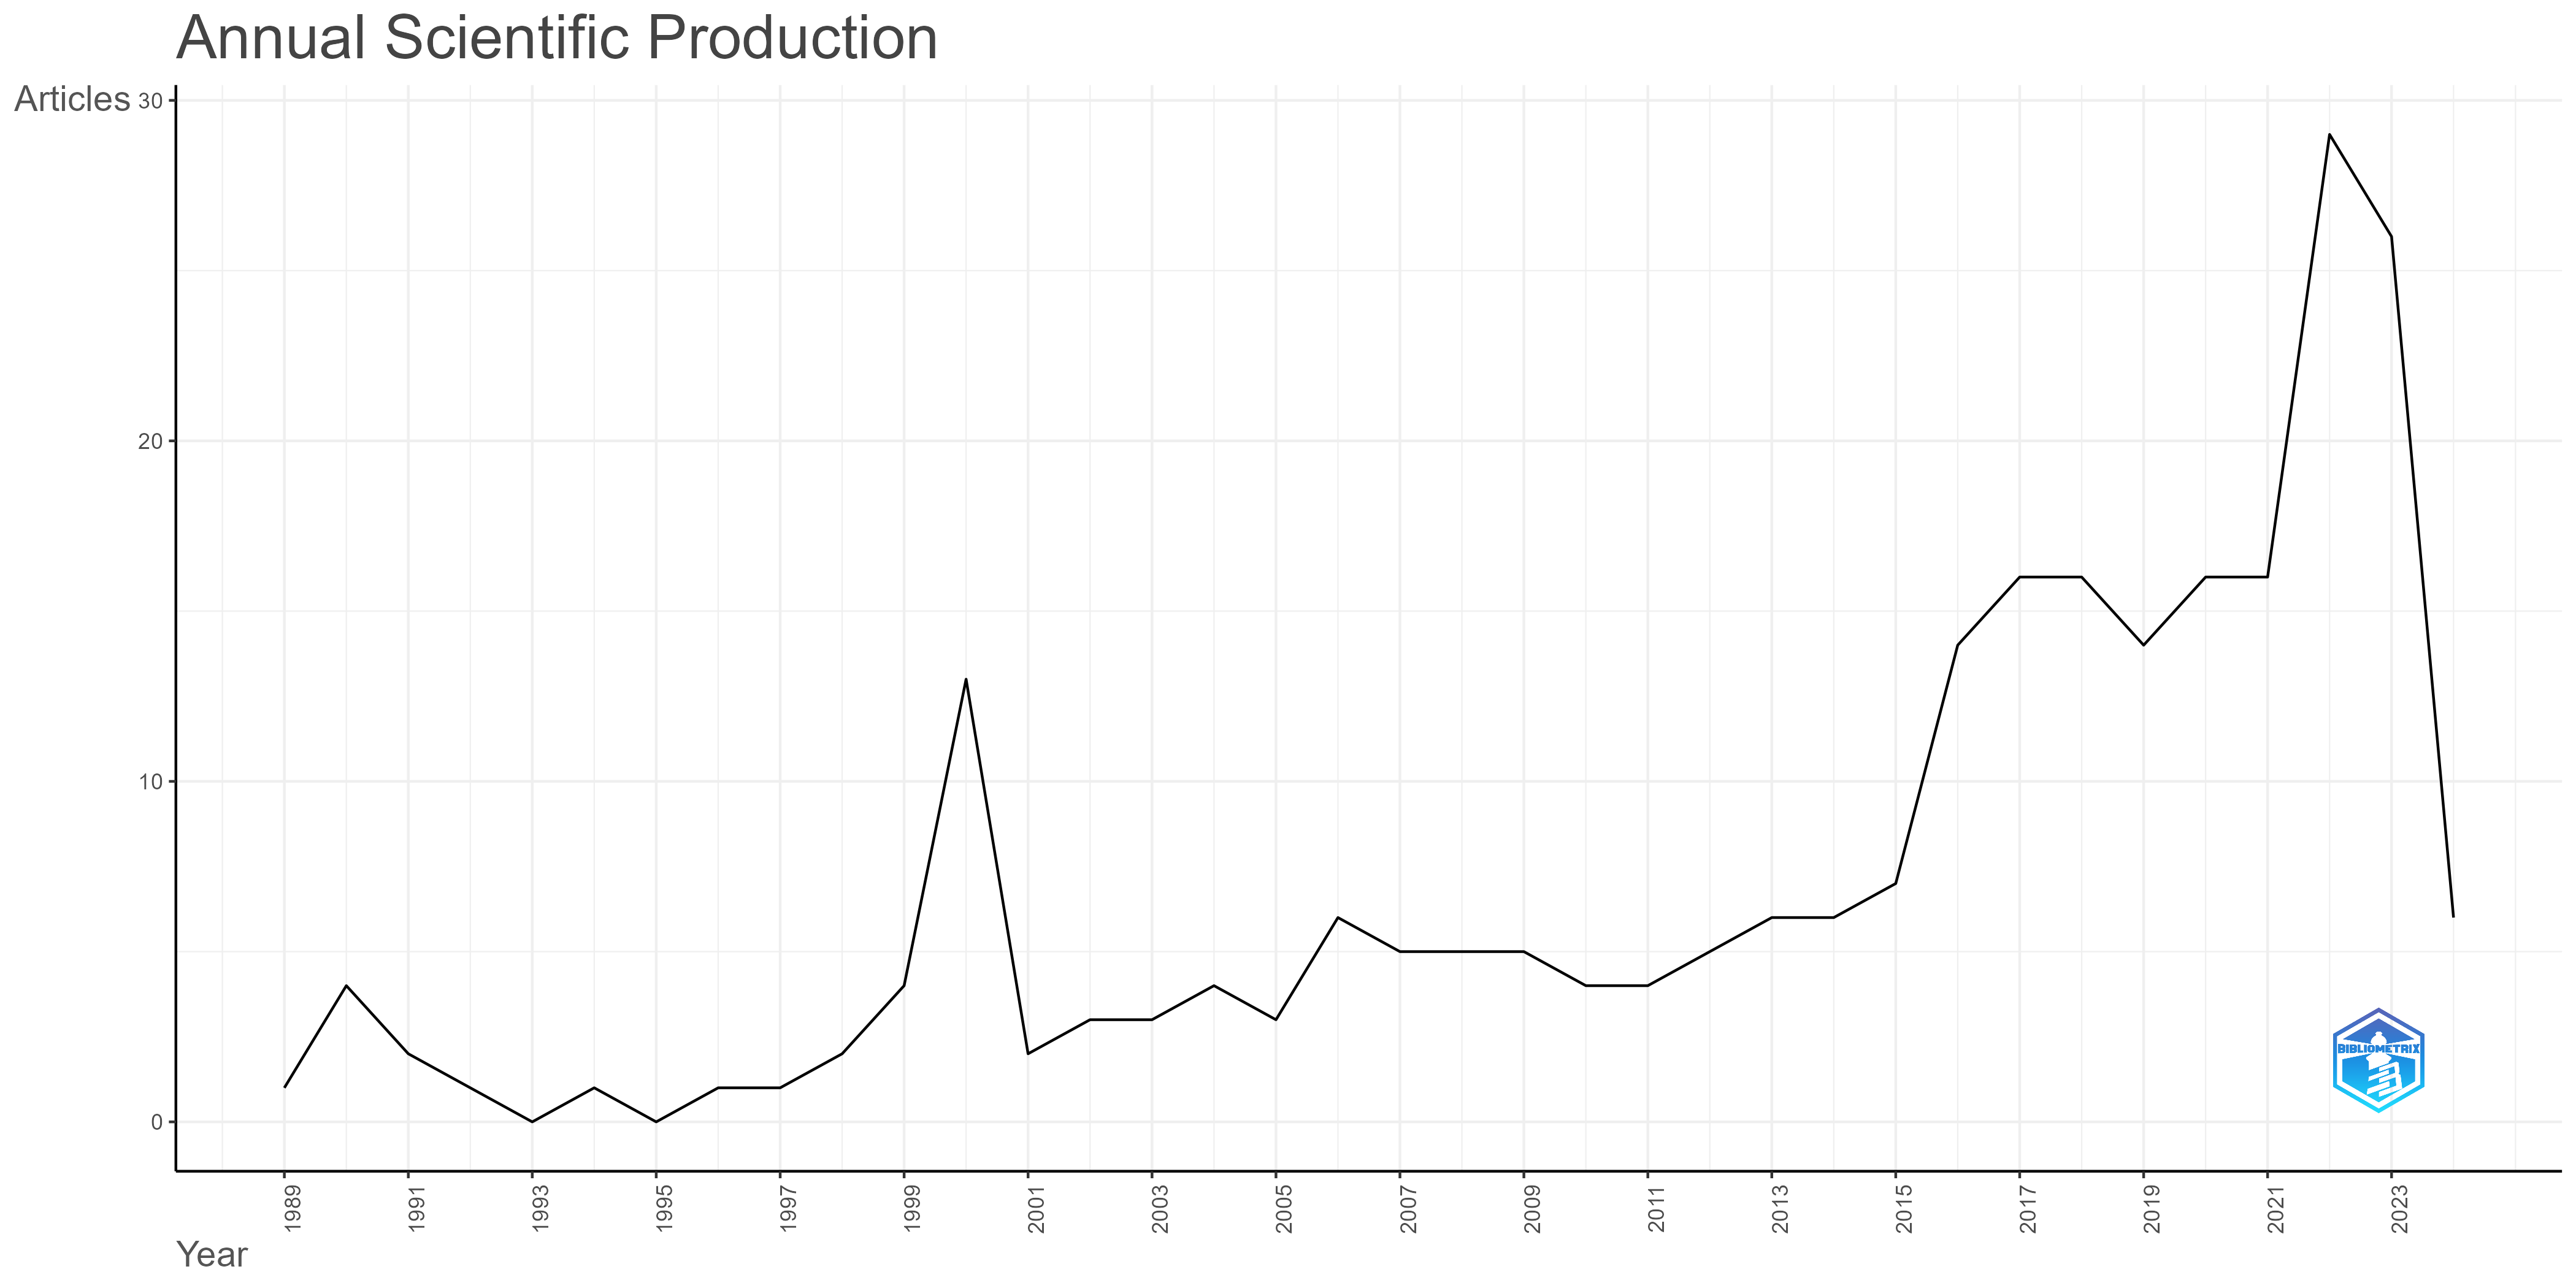
\includegraphics[width=1\linewidth]{AnnualScientificProduction} \caption{Total number of research articles per year that relate to fisheries, mangroves, biomass and biodiversity. \label{AnnualScientificProduction}}\label{fig:AnnualScientificProduction}
\end{figure}



\begin{figure}
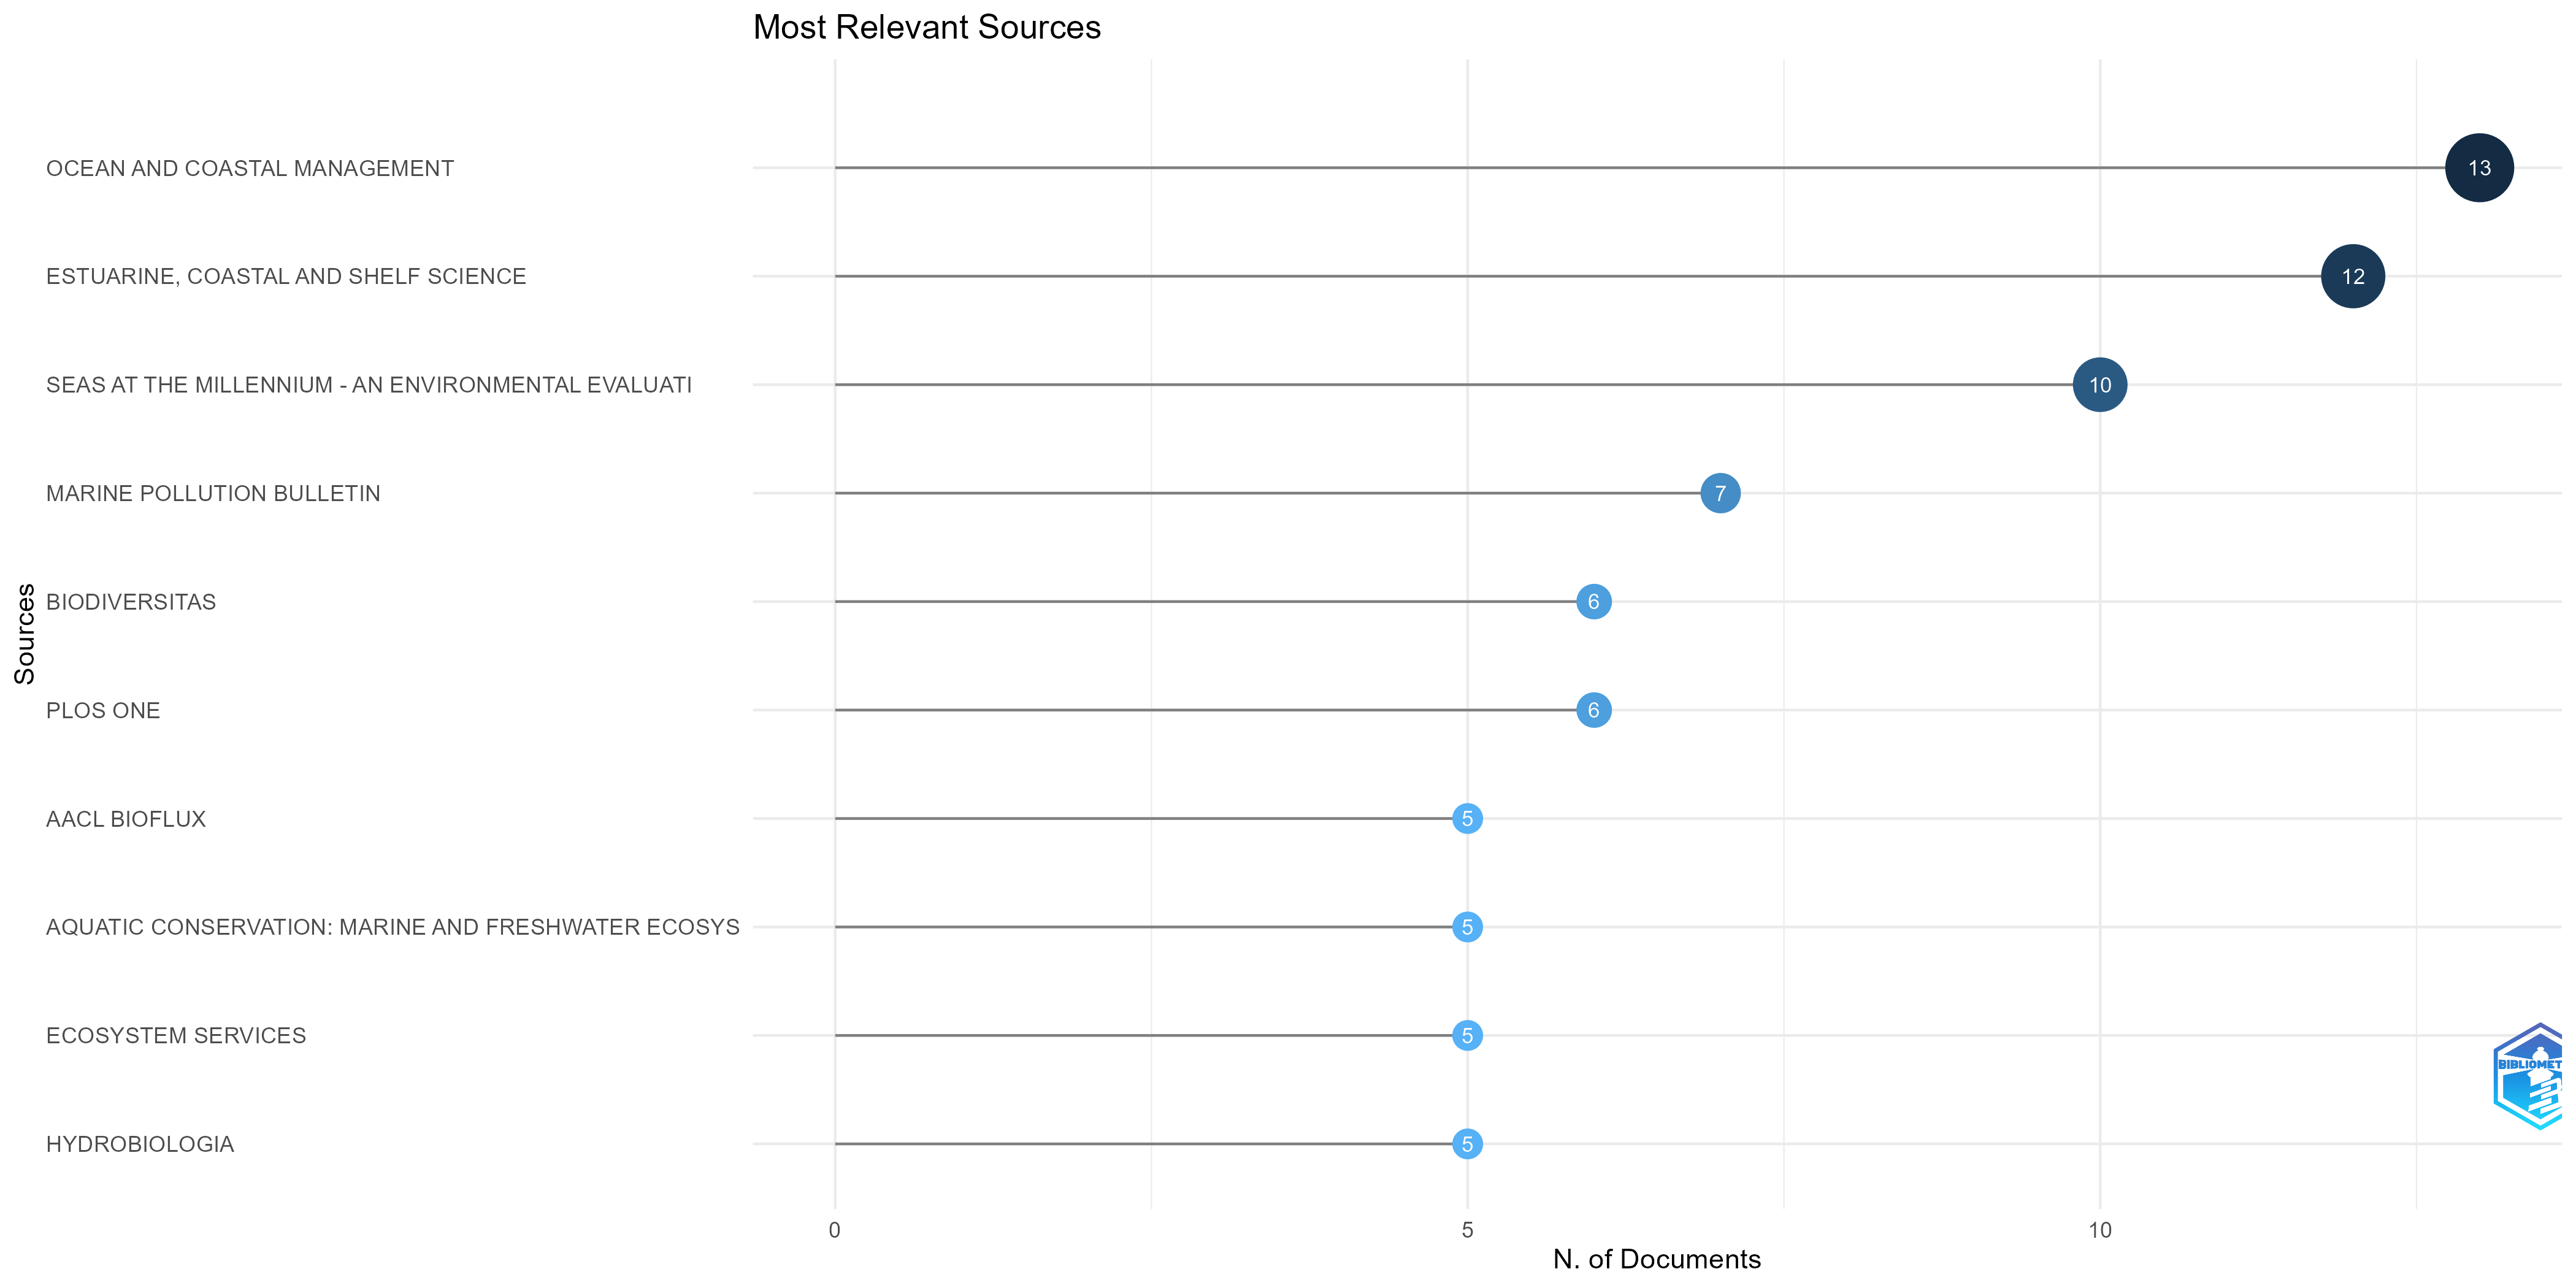
\includegraphics[width=0.5\linewidth]{MostRelevantSources} 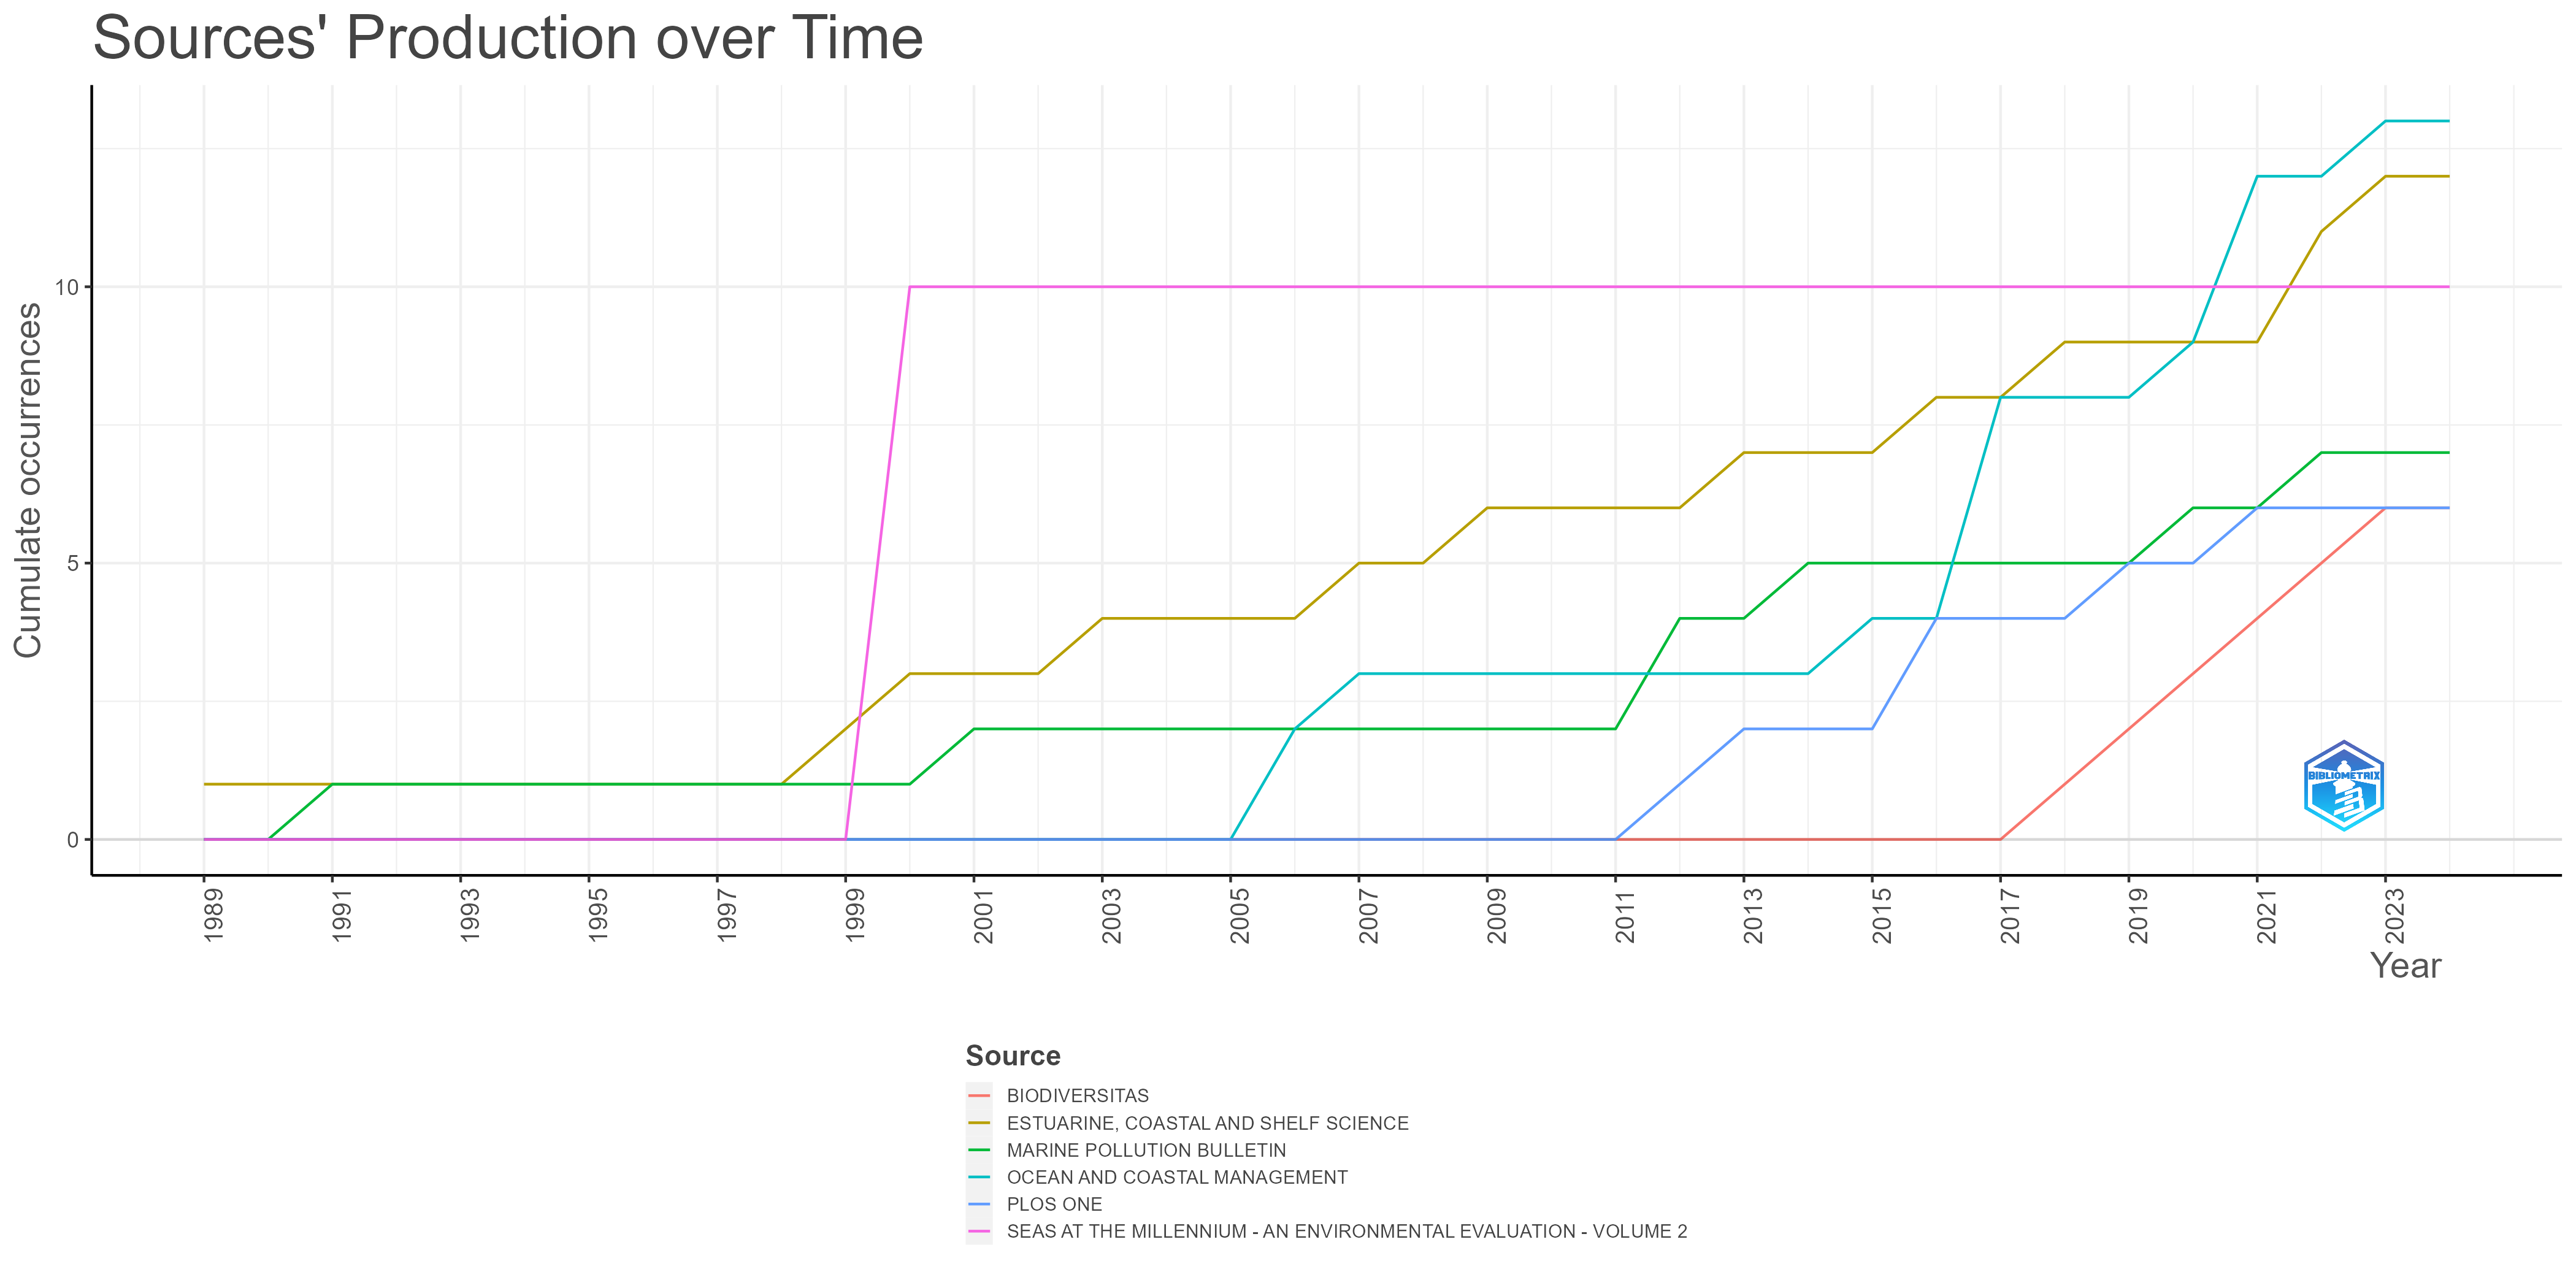
\includegraphics[width=0.5\linewidth]{SourceDynamics} \caption{Total number of publications relating to mangroves, fisheries, and biomass and biodiversity from the top 10 journals (left). Publication trends from the top 6 journals over time (right) \label{SourceDynamics}}\label{fig:SourceDynamics}
\end{figure}



Dates of publication ranged from 1989 to 2024, and 36.65\% of these articles were written with international co-Authorship. Figure \ref{AnnualScientificProduction} shows the total number of articles published which use the keywords of mangroves, fisheries and biomass or biodiversity, ANNUAL GROWTH RATE 5.25\%. The greatest increase in the number of papers written that covers these three topics was in 2015, when the number of articles was 7 to 2016, where the number of articles doubled to 14. The highest number of articles in this analysis was seen in 2022 with 29 articles. This indicates that mangrove and fishery research is increasing in relevance and greater focus on the benefits of mangrove on fisheries worldwide.

The journal that has published the most papers in these areas was Ocean and Coastal Management with 13 total publications. However, this journal's first paper relevant to mangroves, fisheries, and biomass or biodiversity was first published in 2005, whereas Estuarine, Coastal, and Shelf Science, the second most active journal, published its first paper on the subject in 1989 \ref{SourceDynamics}. The journal of Ocean and Coastal Management publishes papers that focus on governance and management issues while the Estuarine, Coastal, and Shelf Science journal covers a broader, more general focus on ocean and estuary science. However, Seas at the Millennium, the journal with the third most papers, was a one-time journal published at the turn of the century that provided a comprehensive review of the environmental condition of the seas of the world. The top six journals that have published on mangroves, fisheries, and biomass or biodiversity all require publications to be made in English.

\begin{figure}
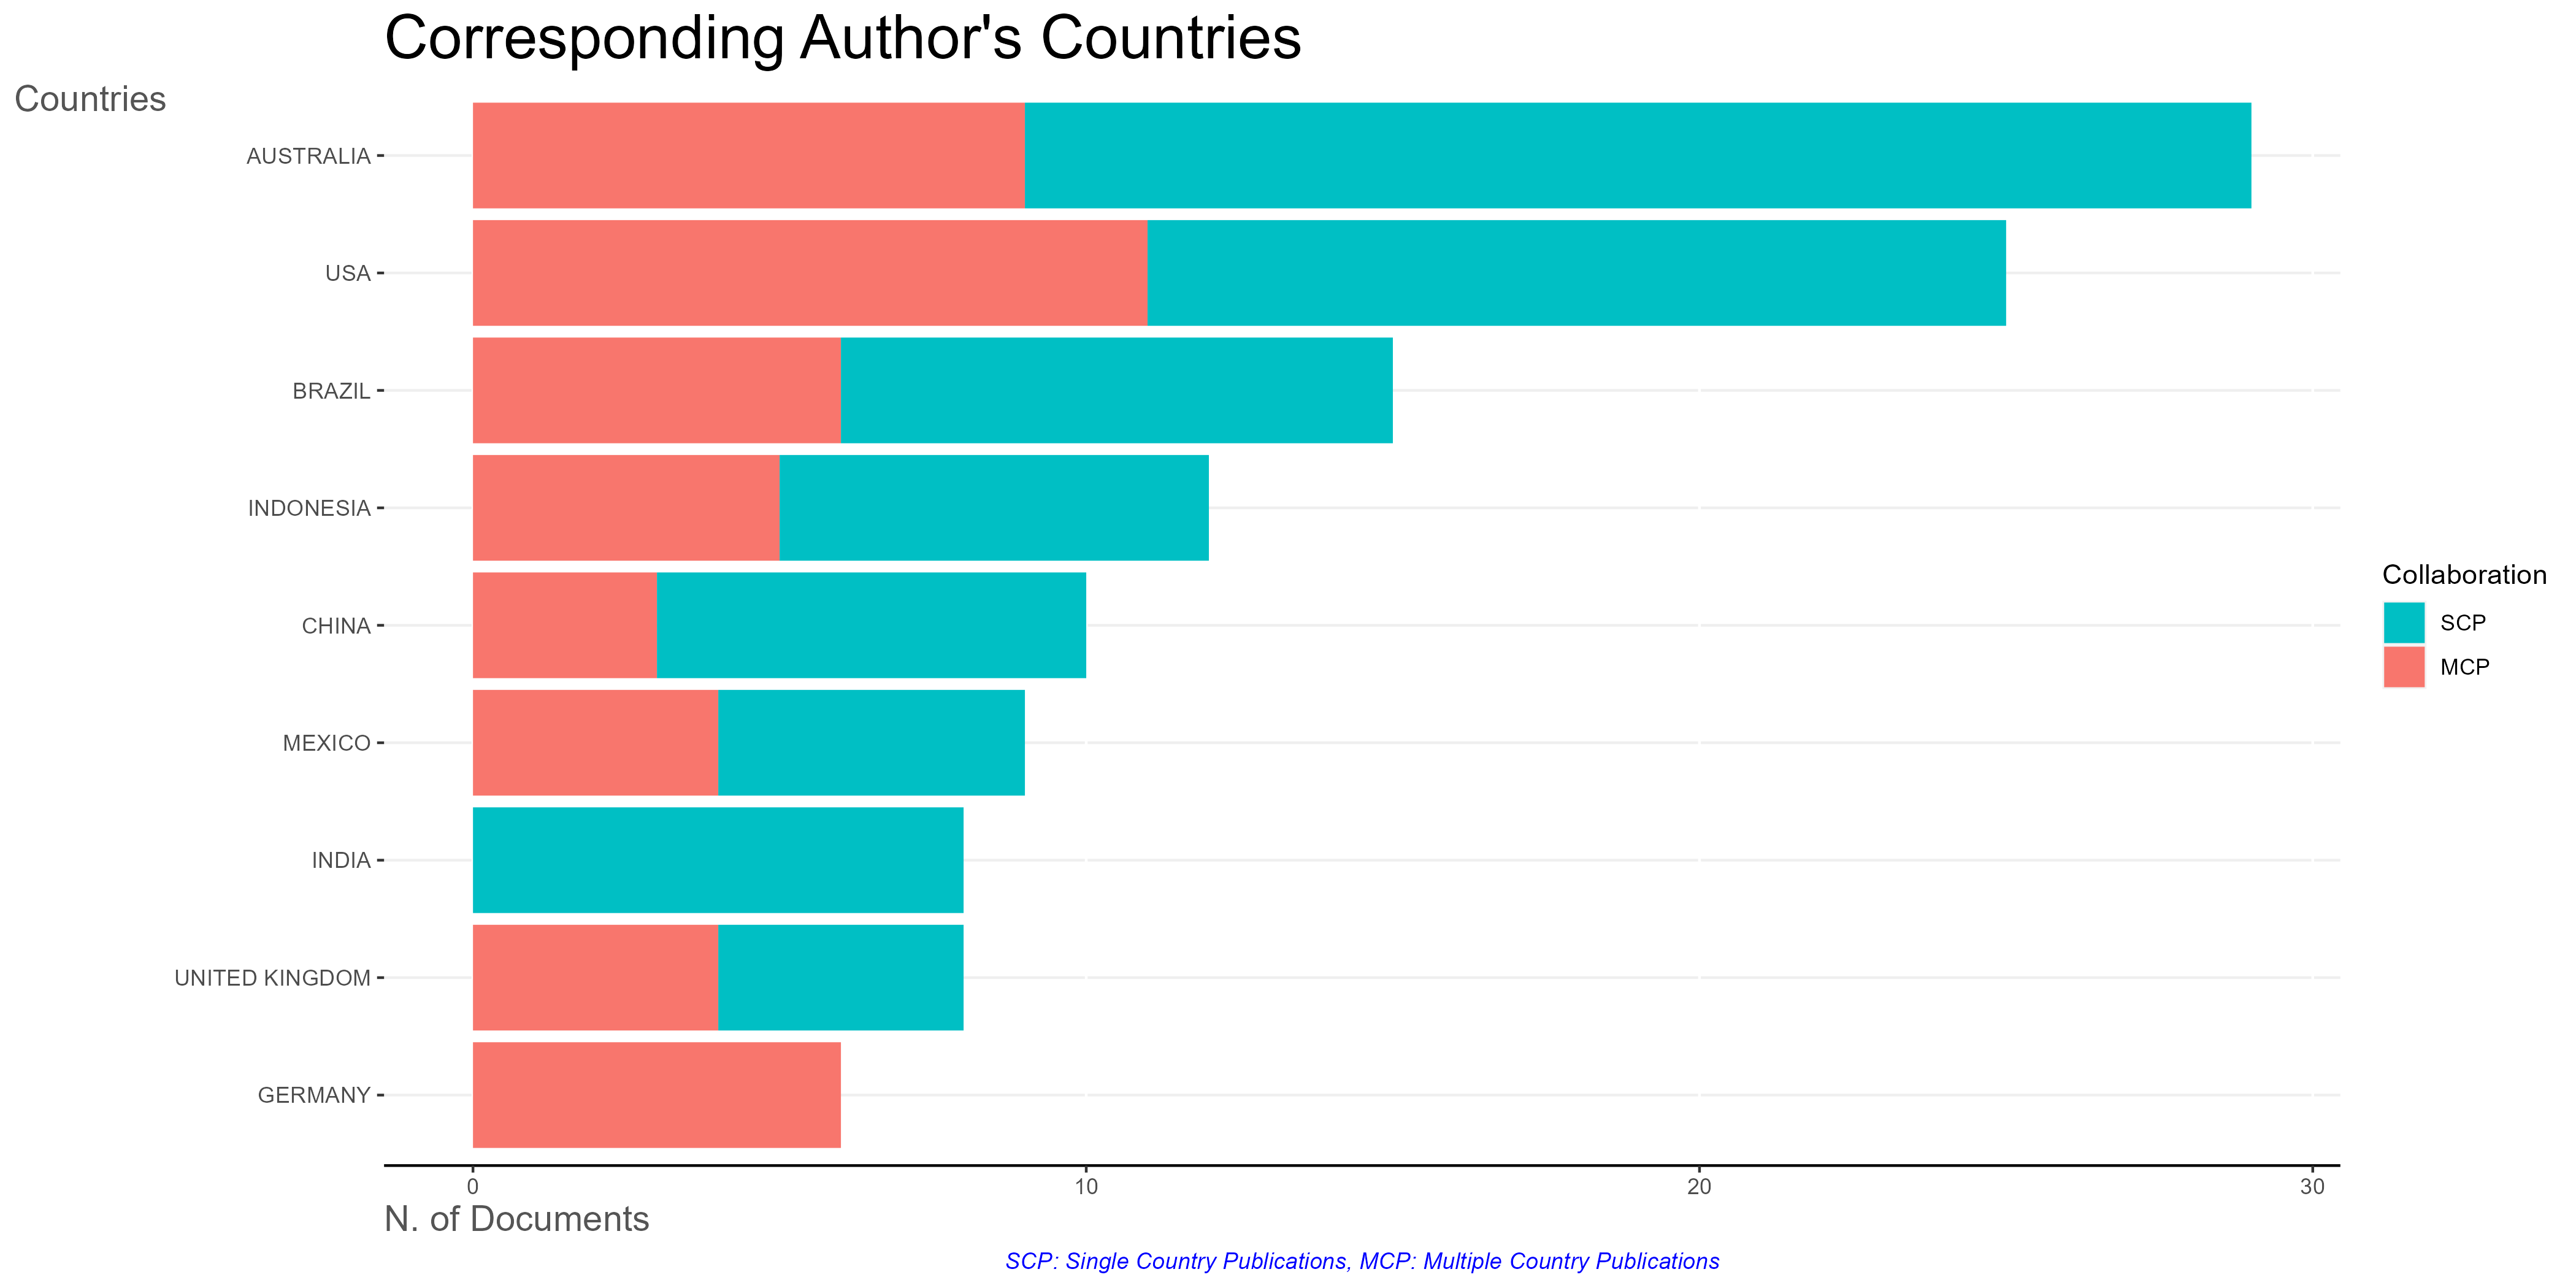
\includegraphics[width=1\linewidth]{AuthorCountries} \caption{Authors' country of origin of documents written from both single country publications (SCP) and multiple country publications (MCP). \label{AuthorCountries}}\label{fig:AuthorCountries}
\end{figure}



\begin{figure}
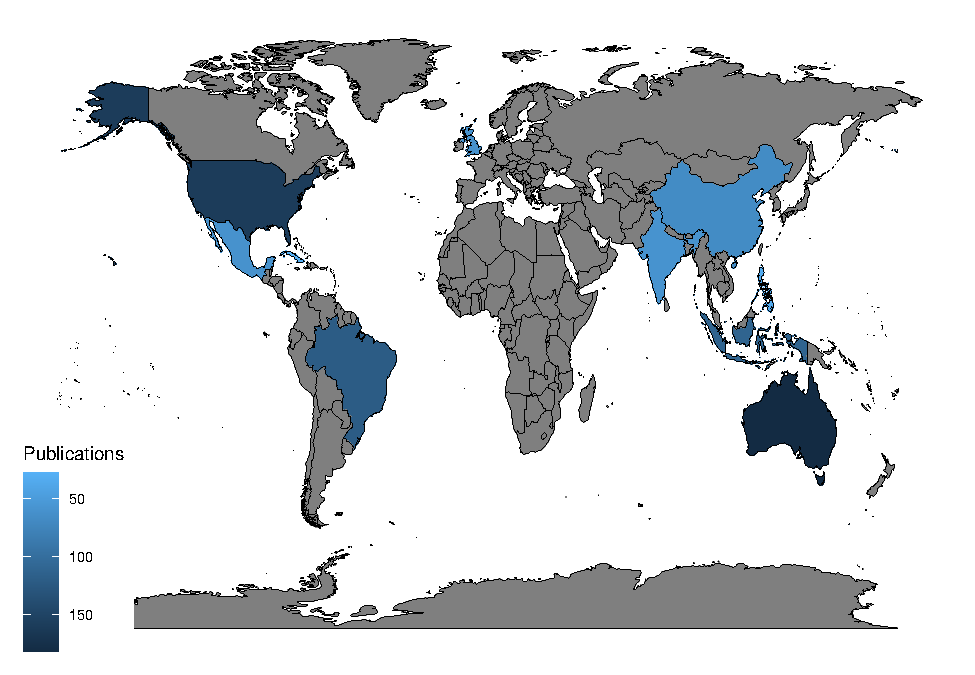
\includegraphics[width=0.5\linewidth]{BibinR_files/figure-latex/countryMap-1} 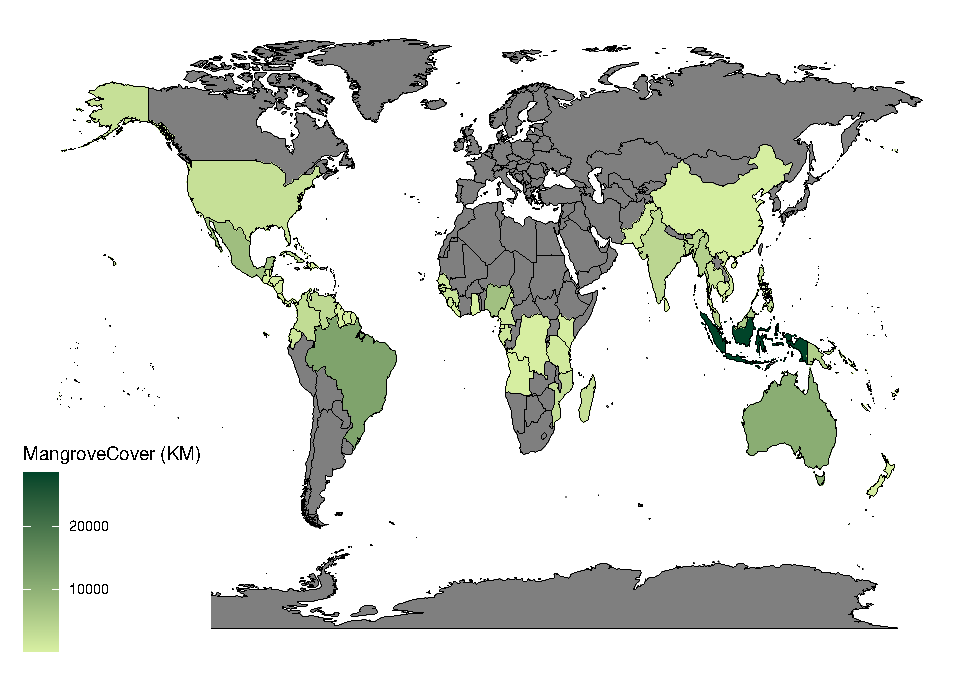
\includegraphics[width=0.5\linewidth]{BibinR_files/figure-latex/countryMap-2} \caption{Number of publications relating to fisheries, mangroves, and biomass or biodiversity (left). Countries with mangrove environments (right) \label{countryMap}}\label{fig:countryMap}
\end{figure}



\begin{figure}
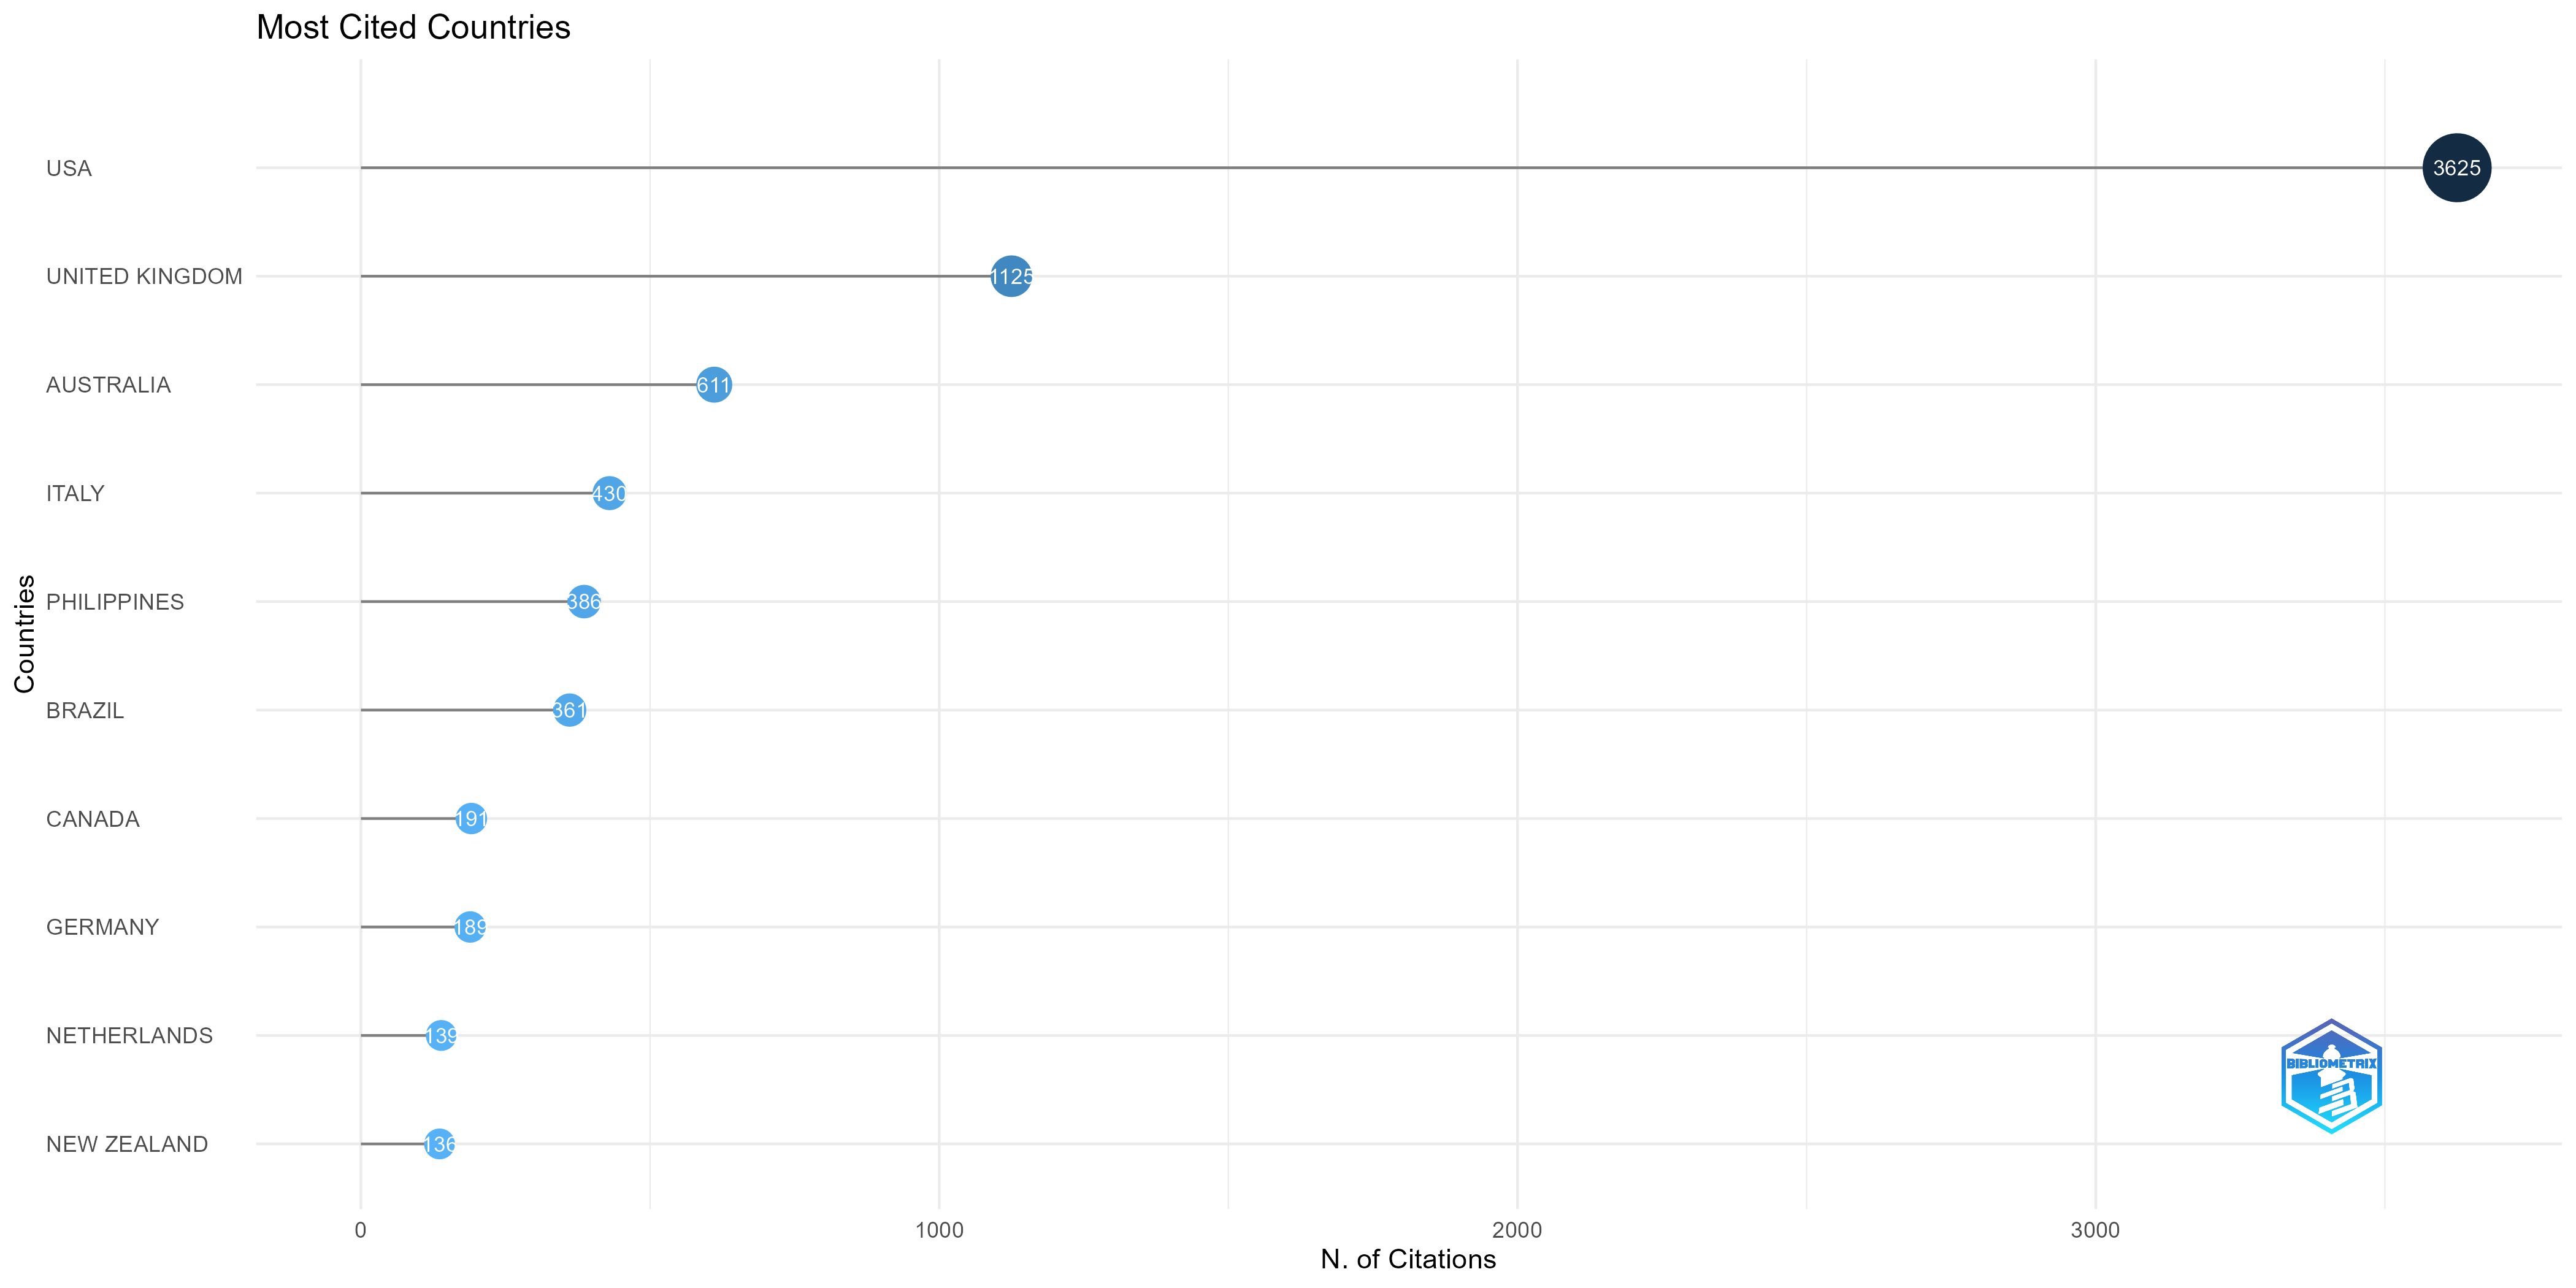
\includegraphics[width=1\linewidth]{MostCitedCountries} \caption{Top ten most cited countries on articles relating to mangroves, fisheries, biomass and biodiversity \label{MostCitedCountries}}\label{fig:MostCitedCountries}
\end{figure}

\begin{figure}
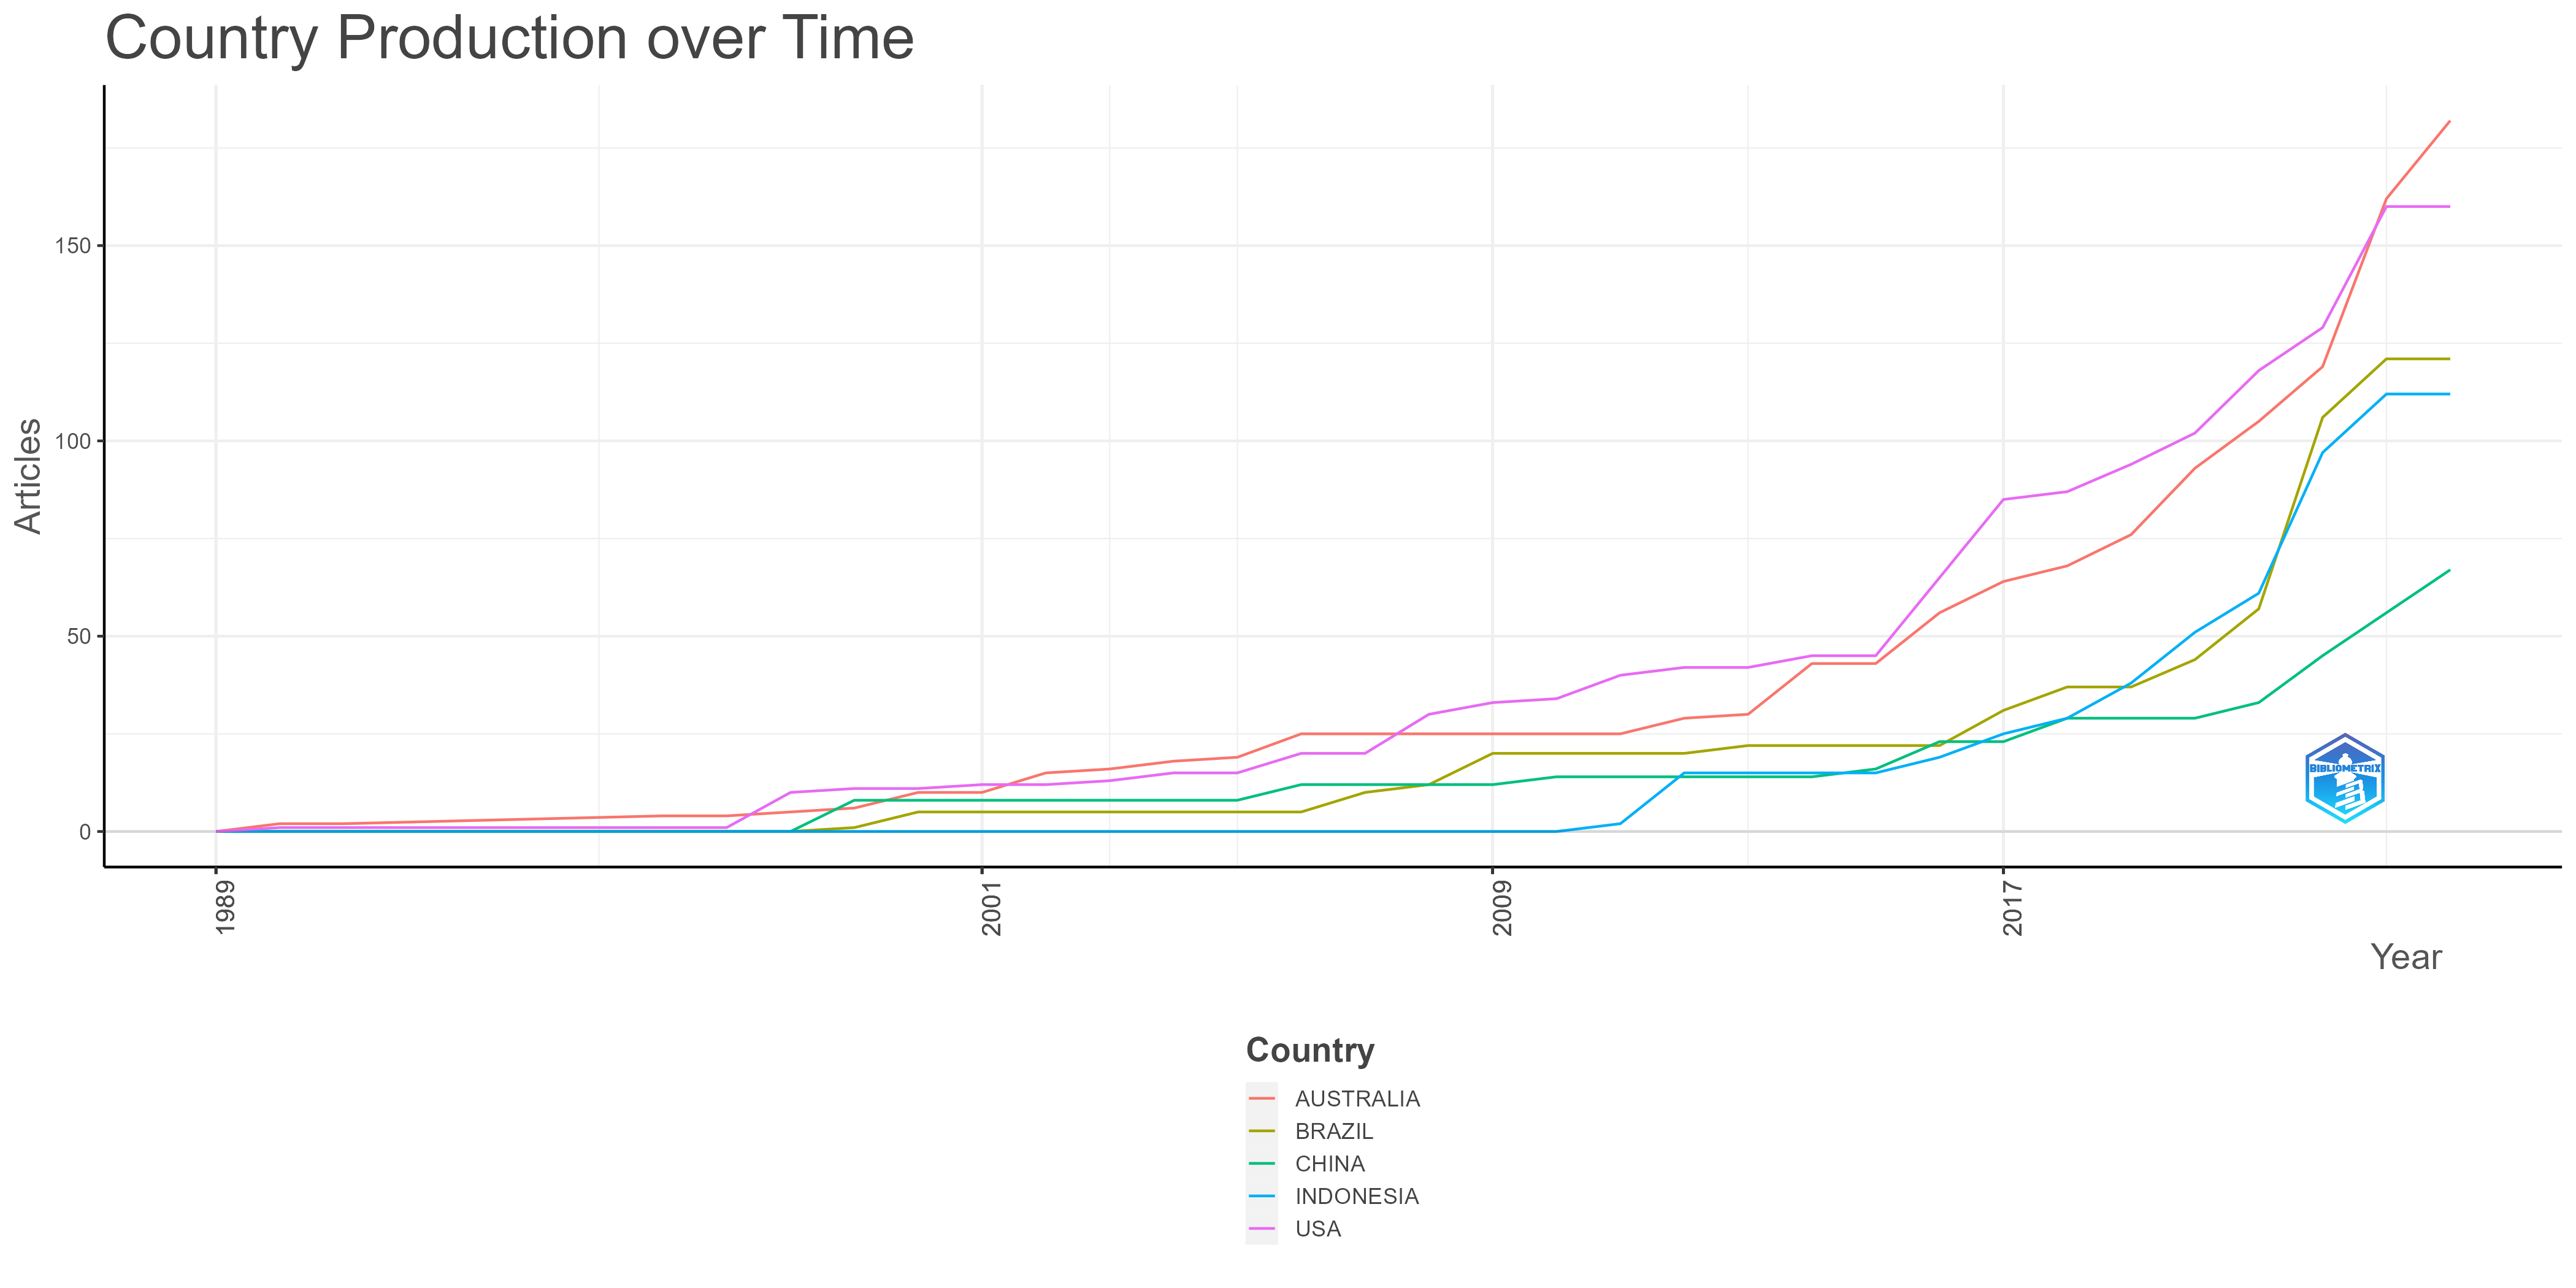
\includegraphics[width=1\linewidth]{CountryOverTime} \caption{Top ten most cited countries on articles relating to mangroves, fisheries, biomass and biodiversity \label{MostCitedCountries}}\label{fig:CountryOverTime}
\end{figure}



In terms of geographic distribution of research on mangroves, fisheries, and biomass or biodiversity, Australia has the highest number of total authorship as well as the highest number of secondary authorship whereas the country with the most Main Corresponding authors is the United States. The United States also has the highest number of cited documents, with 3,681 total citations (Figure \ref{AuthorCountries}). Figure \ref{countryMap} shows the difference between the countries with the most publications relating to mangroves, fisheries, and biomass or biodiversity and compared to the amount of mangrove cover each country has (Jia et al., 2023.) The United States is the most cited country in this area (Figure \ref{MostCitedCountries}), with over three times the number of citations as the United Kingdom, country with the second highest number of citations.

\begin{figure}
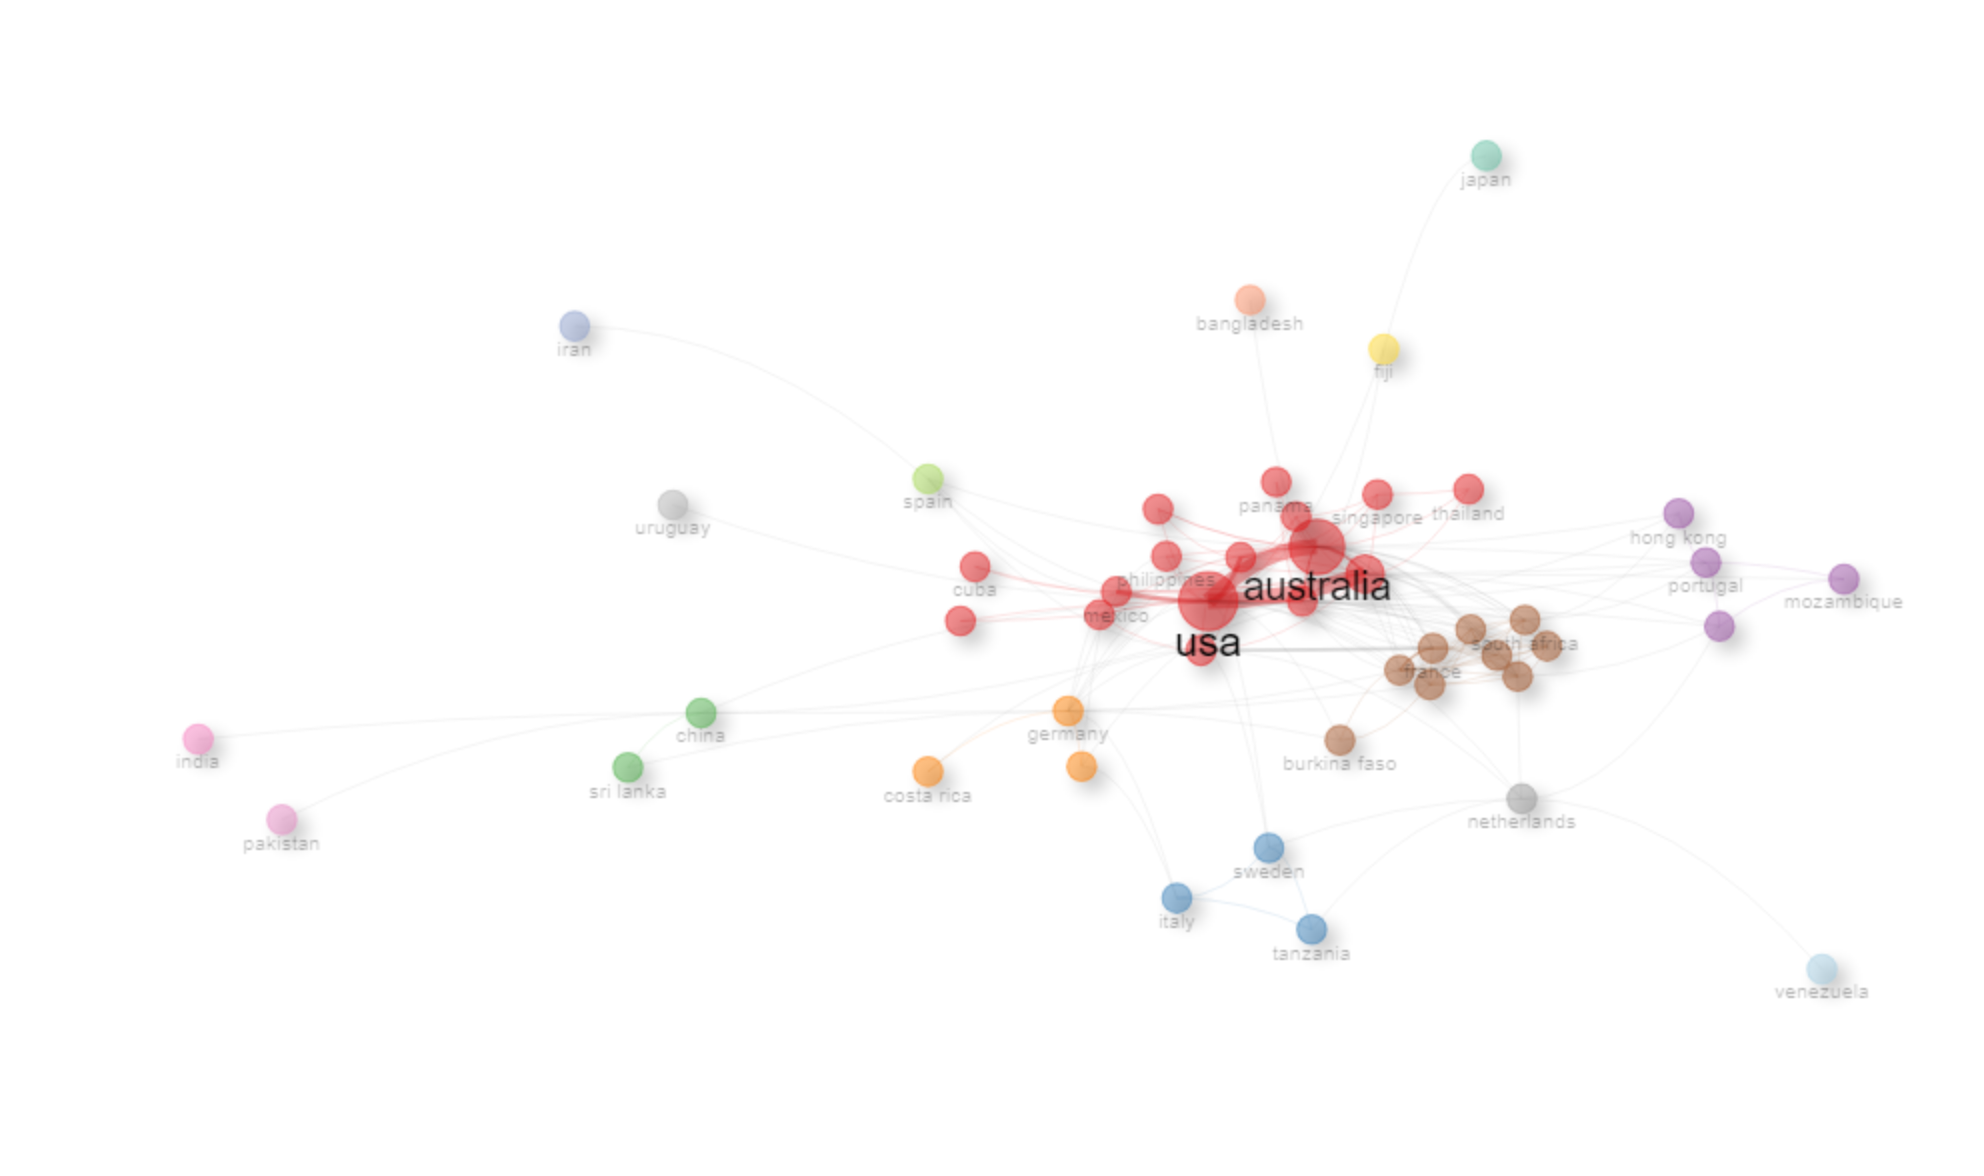
\includegraphics[width=1\linewidth]{CountryCollaborationNetwork} \caption{Network of each country's collaboration with eachother, larger nodes mean a higher number of publications while thicker edges represent higher numbers of collaborations. \label{CountryCollaborationNetwork}}\label{fig:CountryCollaborationNetwork}
\end{figure}



Figure \ref{CountryCollaborationNetwork} shows the amount of authorship collaboration that occurs between each country. By far, the greatest amount of authorship collaboration that occurs is between the US and Australia. Australia has the 3rd largest area of mangroves in the world as of 2020, and the United States has the 19th largest area (Jia et al., 2023).

\begin{figure}
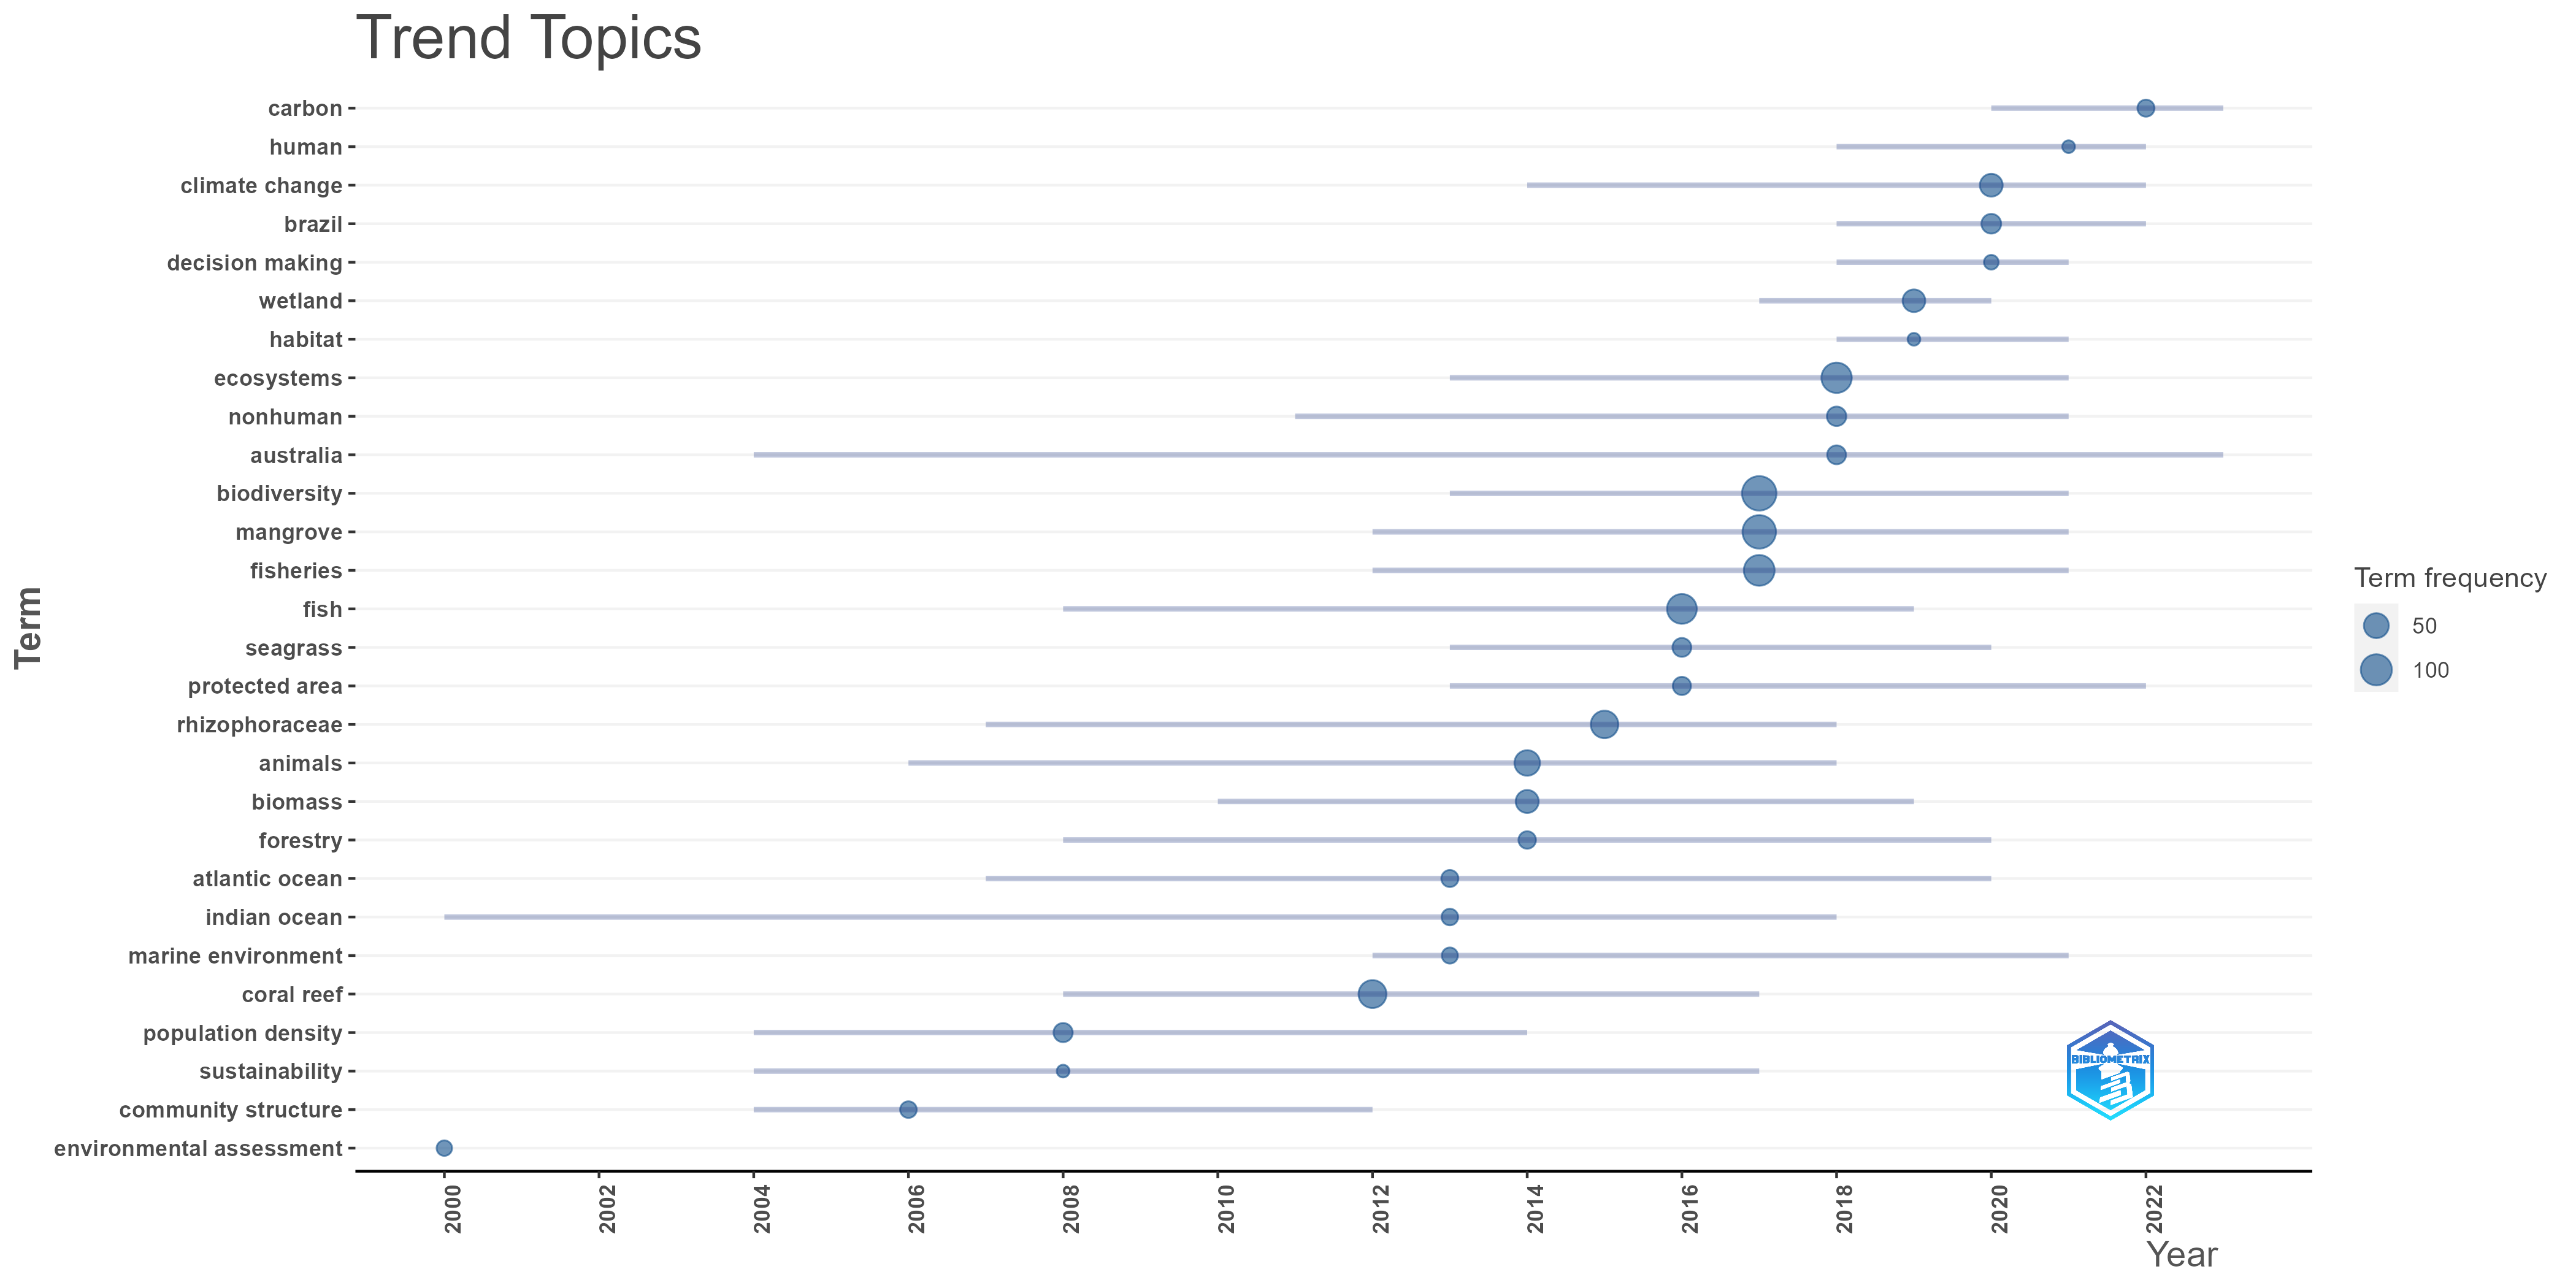
\includegraphics[width=1\linewidth]{TrendTopics} \caption{Trending topics covered by papers relating to mangroves, fisheries, and biomass or biodiversity. The keywords on the left represent words used more than ten times total since 2000. \label{TrendTopics}}\label{fig:TrendTopics}
\end{figure}



Keyword trends are helpful indicators of what issues are relevant when studying mangroves, fisheries. Figure \ref{TrendTopics}shows the most relevant keywords (used more than ten times total and over three times a year) and which years they have been the most used. Most recently, the terms carbon, human, and climate change have become the most relevant topics. Keywords Australia and Indian Ocean both have the longest span of relevancy.

\hypertarget{discussion}{%
\section{DISCUSSION}\label{discussion}}

\newpage

\hypertarget{refs}{}
\begin{CSLReferences}{1}{2}
\leavevmode\vadjust pre{\hypertarget{ref-aburto-oropezaMangrovesGulfCalifornia2008}{}}%
Aburto-Oropeza, O., Ezcurra, E., Danemann, G., Valdez, V., Murray, J., \& Sala, E. (2008). Mangroves in the {Gulf} of {California} increase fishery yields. \emph{Proceedings of the National Academy of Sciences}, \emph{105}(30), 10456--10459. \url{https://doi.org/10.1073/pnas.0804601105}

\leavevmode\vadjust pre{\hypertarget{ref-adeelAssessmentManagementMangrove2002}{}}%
Adeel, Z., \& Pomeroy, R. (2002). Assessment and management of mangrove ecosystems in developing countries. \emph{Trees}, \emph{16}(2-3), 235--238. \url{https://doi.org/10.1007/s00468-002-0168-4}

\leavevmode\vadjust pre{\hypertarget{ref-alongiMangroveForestsResilience2008}{}}%
Alongi, D. M. (2008). Mangrove forests: {Resilience}, protection from tsunamis, and responses to global climate change. \emph{Estuarine, Coastal and Shelf Science}, \emph{76}(1), 1--13. \url{https://doi.org/10.1016/j.ecss.2007.08.024}

\leavevmode\vadjust pre{\hypertarget{ref-alongiCarbonSequestrationMangrove2012}{}}%
Alongi, D. M. (2012). Carbon sequestration in mangrove forests. \emph{Carbon Management}, \emph{3}(3), 313--322. \url{https://doi.org/10.4155/cmt.12.20}

\leavevmode\vadjust pre{\hypertarget{ref-blueforestsAdaptiveCollaborativeManagement2012new}{}}%
Blue Forests. (2012). \emph{Adaptive {Collaborative} {Management} {Plan} for {Building} {Mangrove} {Resilience} in {Tanakeke} {Island}}.

\leavevmode\vadjust pre{\hypertarget{ref-cameronEstimatingFullGreenhouse2019}{}}%
Cameron, C., Hutley, L. B., \& Friess, D. A. (2019). Estimating the full greenhouse gas emissions offset potential and profile between rehabilitating and established mangroves. \emph{Science of The Total Environment}, \emph{665}, 419--431. \url{https://doi.org/10.1016/j.scitotenv.2019.02.104}

\leavevmode\vadjust pre{\hypertarget{ref-carugatiImpactMangroveForests2018}{}}%
Carugati, L., Gatto, B., Rastelli, E., Lo Martire, M., Coral, C., Greco, S., \& Danovaro, R. (2018). Impact of mangrove forests degradation on biodiversity and ecosystem functioning. \emph{Scientific Reports}, \emph{8}(1), 13298. \url{https://doi.org/10.1038/s41598-018-31683-0}

\leavevmode\vadjust pre{\hypertarget{ref-donthuHowConductBibliometric2021}{}}%
Donthu, N., Kumar, S., Mukherjee, D., Pandey, N., \& Lim, W. M. (2021). How to conduct a bibliometric analysis: {An} overview and guidelines. \emph{Journal of Business Research}, \emph{133}, 285--296. \url{https://doi.org/10.1016/j.jbusres.2021.04.070}

\leavevmode\vadjust pre{\hypertarget{ref-ellegaardBibliometricAnalysisScholarly2015}{}}%
Ellegaard, O., \& Wallin, J. A. (2015). The bibliometric analysis of scholarly production: {How} great is the impact? \emph{Scientometrics}, \emph{105}(3), 1809--1831. \url{https://doi.org/10.1007/s11192-015-1645-z}

\leavevmode\vadjust pre{\hypertarget{ref-ellisonOriginsMangroveEcosystems1999}{}}%
Ellison, A. M., Farnsworth, E. J., \& Merkt, R. E. (1999). Origins of mangrove ecosystems and the mangrove biodiversity anomaly: {Mangrove} biodiversity anomaly. \emph{Global Ecology and Biogeography}, \emph{8}(2), 95--115. \url{https://doi.org/10.1046/j.1466-822X.1999.00126.x}

\leavevmode\vadjust pre{\hypertarget{ref-gilmanThreatsMangrovesClimate2008}{}}%
Gilman, E. L., Ellison, J., Duke, N. C., \& Field, C. (2008). Threats to mangroves from climate change and adaptation options: {A} review. \emph{Aquatic Botany}, \emph{89}(2), 237--250. \url{https://doi.org/10.1016/j.aquabot.2007.12.009}

\leavevmode\vadjust pre{\hypertarget{ref-hutchisonRoleMangrovesFisheries2014}{}}%
Hutchison, J., \& Spalding, M. (2014). The {Role} of {Mangroves} in {Fisheries Enhancement}. \emph{The Nature Conservancy and Wetlands International.}

\leavevmode\vadjust pre{\hypertarget{ref-jiaMappingGlobalDistribution2023}{}}%
Jia, M., Wang, Z., Mao, D., Ren, C., Song, K., Zhao, C., Wang, C., Xiao, X., \& Wang, Y. (2023). Mapping global distribution of mangrove forests at 10-m resolution. \emph{Science Bulletin}, \emph{68}(12), 1306--1316. \url{https://doi.org/10.1016/j.scib.2023.05.004}

\leavevmode\vadjust pre{\hypertarget{ref-nagelkerkenHabitatFunctionMangroves2008}{}}%
Nagelkerken, I., Blaber, S. J. M., Bouillon, S., Green, P., Haywood, M., Kirton, L. G., Meynecke, J.-O., Pawlik, J., Penrose, H. M., Sasekumar, A., \& Somerfield, P. J. (2008). The habitat function of mangroves for terrestrial and marine fauna: {A} review. \emph{Aquatic Botany}, \emph{89}(2), 155--185. \url{https://doi.org/10.1016/j.aquabot.2007.12.007}

\leavevmode\vadjust pre{\hypertarget{ref-zuermgassenReprintFishersWho2021}{}}%
Zu Ermgassen, P. S. E., Mukherjee, N., Worthington, T. A., Acosta, A., Rocha Araujo, A. R. D., Beitl, C. M., Castellanos-Galindo, G. A., Cunha-Lignon, M., Dahdouh-Guebas, F., Diele, K., Parrett, C. L., Dwyer, P. G., Gair, J. R., Johnson, A. F., Kuguru, B., Savio Lobo, A., Loneragan, N. R., Longley-Wood, K., Mendonça, J. T., \ldots{} Spalding, M. (2021). Reprint of : {Fishers} who rely on mangroves: {Modelling} and mapping the global intensity of mangrove-associated fisheries. \emph{Estuarine, Coastal and Shelf Science}, \emph{248}, 107159. \url{https://doi.org/10.1016/j.ecss.2020.107159}

\end{CSLReferences}

\end{document}
